\section{Environmental Impacts}\label{environmental-impacts}

Typically when a new building technology is evaluated the energy performance of a baseline building is compared to the energy and life-cycle costs of alternatives to determine cost-effectiveness. But what if the lowest energy or life-cycle cost alternative is not the cleanest or lowest environmental impact?~ By calculating environmental impact, designers can compare alternatives not only in terms of their energy performance but also their environmental performance---working towards a more sustainable design (Liesen 1997; Stroot, Nemeth, and Fournier 1996).~ Environmental impacts are quantified, in part, by modeling the amount of emissions and in EnergyPlus this is done using the input objects ``EnvironmentalImpactFactors,'' ``FuelFactors,'' and ``Output:EnvironmentalImpactFactors.''

Based on emissions factors entered by the user, EnergyPlus calculates the mass or volume of thirteen different pollutants: CO\(_{2}\) (carbon dioxide), CO (carbon monoxide), CH\(_{4}\) (methane), NO\(_{x}\) (nitrogen oxides), N\(_{2}\)O (nitrous oxide), SO\(_{2}\) (sulphur dioxide), PM (particulate matter), PM\(_{10}\) (particulate matter 10\textgreater{}PM\(_{10}\)\textgreater{}2.5 microns), PM\(_{2.5}\) (particulate matter\textless{}2.5 microns), NH\(_{3}\) (ammonia), NMVOC (non-methane volatile organic compounds), Hg (mercury), and Pb (lead) as well as water consumed through evaporation in thermo- and hydro-electric generation and high- and low-level nuclear waste from nuclear electricity generation for on- and off-site energy production.~ Note that while these comprise the largest proportion of pollutants, more than one hundred other pollutants are emitted from fossil fuel combustion or electricity generation. Much of the information compiled here for fossil fuel combustion comes from \emph{AP-42 Compilation of Air Pollutant Emission Factors} (EPA 1998a, 1998b, 1996).~ For more information on pollutants, see the U.S. Environmental Protection Agency (EPA) Clearinghouse for Inventories \& Emission Factors (\href{http://www.epa.gov/ttn/chief/efinformation.html}{www.epa.gov/ttn/chief/efinformation.html}).

EnergyPlus models energy performance of on-site fossil fuels and purchased electricity (generated from a variety of fuels including natural gas, oil, gasoline, diesel, coal, hydroelectric, nuclear, wind, solar power, and biomass).~ The energy performance calculated by EnergyPlus is converted into a mass or volume of pollutants emitted.~ From a baseline building, alternative energy and pollution saving technologies can be explored, and the energy savings and pollution reduction can be calculated.~ Figure~\ref{fig:example-annual-atmospheric-pollutants} and Figure~\ref{fig:example-annual-total-carbon-equivalent-for} illustrate a comparison of two buildings simulated using Chicago weather data in EnergyPlus and the calculated pollutant levels (based on U.S. national average pollutants) (Crawley 2003).

To calculate the mass or volume of each pollutant, consumption is multiplied by an emissions factor for each fuel (natural gas, electricity, fuel oil, diesel, or coal). In future versions, users will be able to schedule how the emissions factors by time of day, month, season and year.~ For electricity, the mix of generation fuel sources---whether utility, state or regional---is used to adjust the emission factors. ~If a user has emissions factors specific to the building site and equipment, these can be entered directly.~ \textbf{There are no default emissions factors}.

\subsection{Types of Pollutants}\label{types-of-pollutants}

EPA categorizes pollutants as either Criteria Pollutants or Hazardous Pollutants. Criteria pollutants are the six substances for which EPA has set health-based standards, including carbon monoxide (CO), nitrogen oxides (NO\(_{x}\)), sulfur dioxide (SO\(_{2}\)), and particulate matter (PM10 and PM2.5), ozone (O\(_{3}\)), and lead (Pb).~ Because ozone is created in atmospheric photochemical reactions of volatile organic compounds, ammonia, and other substances rather than direct building-related energy emissions, we do not calculated ozone emissions in EnergyPlus.~ But we do include ozone precursors: methane (CH\(_{4}\)), non-methane volatile organic compounds (NMVOC), and ammonia (NH\(_{3}\)). Hazardous pollutants are substances that are known or suspected to cause serious health problems such as cancer.~ We include typical hazardous substances associated with energy production and use including lead (Pb) and mercury (Hg). We also include CO\(_{2}\) (carbon dioxide) since it is largest greenhouse gas in terms of impact.

\begin{figure}[hbtp] % fig 341
\centering
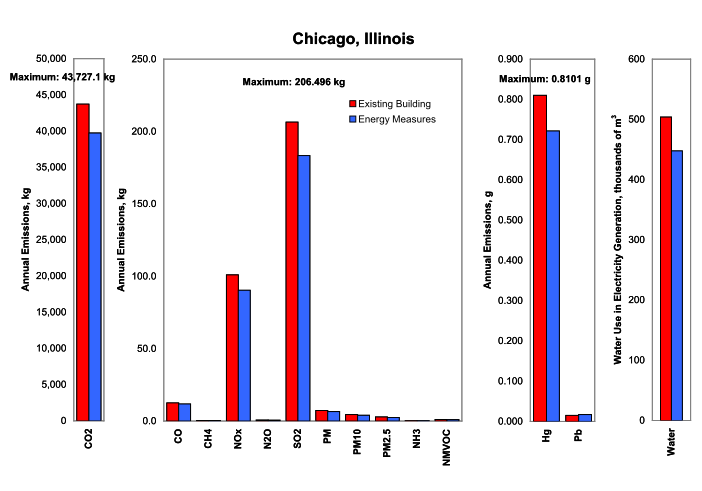
\includegraphics[width=0.9\textwidth, height=0.9\textheight, keepaspectratio=true]{media/image7910.svg.png}
\caption{Example Annual Atmospheric Pollutants and Water Consumption \protect \label{fig:example-annual-atmospheric-pollutants}}
\end{figure}

\begin{figure}[hbtp] % fig 342
\centering
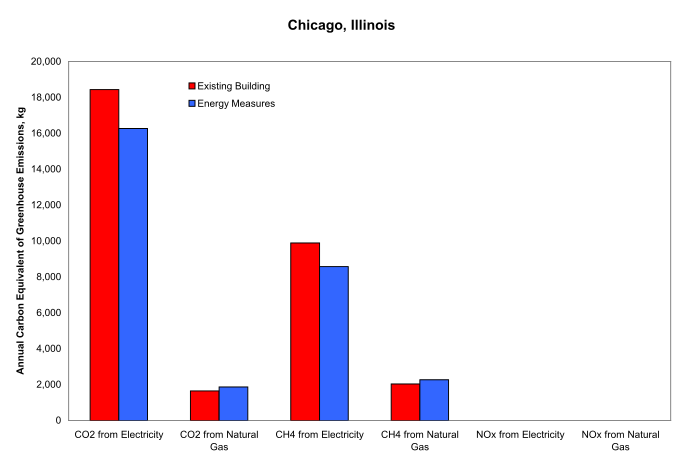
\includegraphics[width=0.9\textwidth, height=0.9\textheight, keepaspectratio=true]{media/image7911.svg.png}
\caption{Example Annual Total Carbon Equivalent for Major Greenhouse Gases \protect \label{fig:example-annual-total-carbon-equivalent-for}}
\end{figure}

\subsection{Carbon Equivalent}\label{carbon-equivalent}

The Intergovernmental Panel on Climate Change has studied the effects on the relative radiative forcing effects of various greenhouse gases.~ This effect, called Global Warming Potential (GWP), is described in terms of the Carbon Equivalent of a particular greenhouse gas.~ This equivalent is based on a factor of 1.0 for carbon.~ This group of gases includes carbon dioxide (CO\(_{2}\)), carbon monoxide, nitrous oxide, methane, halocarbon emission, hydrofluorocarbons (HFC), perfluorocarbons (PFC), and chlorofluorocarbons (CFC).~ For building energy use, the main gases of concern are carbon dioxide, carbon monoxide, methane, and nitrous oxide.~ Although carbon monoxide has a relatively short life, CO emissions into the atmosphere may have a significant impact on climate forcing due to chemical impact on CH\(_{4}\) lifetime, and tropospheric O\(_{3}\) and CO\(_{2}\) photochemical production normally reacts to produce carbon dioxide, but it can't be ignored since it is produced in incomplete combustion and the carbon remains to interact as CO\(_{2}\) Yet there is no agreement on its carbon equivalent (IPCC 2001). The carbon equivalent of carbon dioxide, methane, and nitrous oxide are calculated and then multiplied by their GWP on a 100 year time frame.~ The Carbon Equivalents of the following gases have been determined and used in the program are shown in the following table.

% table 93
\begin{longtable}[c]{@{}lc@{}}
\caption{Carbon Equivalents (IPCC 2001) \label{table:carbon-equivalents-ipcc-2001}} \tabularnewline
\toprule 
Gas & Carbon Equivalent \tabularnewline
\midrule
\endfirsthead

\caption[]{Carbon Equivalents (IPCC 2001)} \tabularnewline
\toprule 
Gas & Carbon Equivalent \tabularnewline
\midrule
\endhead

NO\(_x\) & 80.7272 \tabularnewline
CH\(_4\) & 6.2727 \tabularnewline
CO\(_2\) & 0.2727 \tabularnewline
\bottomrule
\end{longtable}

The resulting carbon equivalents by fuel type are shown in the output of the program along with the individual gas pollutants.

\subsection{Fossil Fuel Emissions Factors}\label{fossil-fuel-emissions-factors}

Emission factors for on-site fossil fuel consumption are based on Section 1.4 Natural Gas Combustion in EPA (1998a) Table~\ref{table:emission-factors-for-natural-gas} shows the greenhouse gas and precursors and criteria pollutant emissions factors for natural gas.~ Similar emissions factors are shown for residual fuel oil (No. 4 and No. 6 fuel oil) {[}Table~\ref{table:emission-factors-for-residual-fuel-oil-no.-4}{]}, distillates (No. 1 and No. 2 fuel oil) {[}Table~\ref{table:emission-factors-for-distillates-no.-1}{]}, residential oil furnace {[}Table~\ref{table:emission-factors-for-residential-oil-furnace}{]}, LPG (butane and propane) {[}Table~\ref{table:emission-factors-for-lpg-butane-and-propane}{]}, gasoline and diesel {[}Table~\ref{table:emission-factors-for-gasoline-and-diesel}{]}, and coal {[}Table~\ref{table:emission-factors-for-coal}{]} in the indicated tables.~ Note that a zero for a pollutant in the table may mean that no data were available, not that there are no emissions of that pollutant.

% table 94
\begin{longtable}[c]{p{4.5in}p{1.5in}}
\caption{Emission Factors for Natural Gas \label{table:emission-factors-for-natural-gas}} \tabularnewline
\toprule 
Pollutant & Emission Factor\(^a\)  ~~ (g/MJ) \tabularnewline
\midrule
\endfirsthead

\caption[]{Emission Factors for Natural Gas} \tabularnewline
\toprule 
Pollutant & Emission Factor\(^a\)  ~~ (g/MJ) \tabularnewline
\midrule
\endhead

Carbon Dioxide (CO\(_2\)) & 50.23439 \tabularnewline
Carbon Monoxide (CO) & 3.51641E-02 \tabularnewline
Methane (CH\(_4\)) & 9.62826E-04 \tabularnewline
Nitrogen Oxides (NO\(_x\)) & 4.18620E-02 \tabularnewline
Nitrous Oxide (N\(_2\)O)\(^b\) & 9.20964E-04 \tabularnewline
Sulphur Dioxide (SO\(_2\))\(^c\) & 2.51172E-04 \tabularnewline
Particulate Matter (PM)\(^d\) & 3.18151E-03 \tabularnewline
Particulate Matter (PM10)\(^d\) & 2.38613E-03 \tabularnewline
Particulate Matter (PM2.5)\(^d\) & 7.95378E-04 \tabularnewline
Ammonia (NH\(_3\)) & 0\(^e\) \tabularnewline
Volatile Organic Compounds (NMVOC) & 2.30241E-03 \tabularnewline
Mercury (Hg) & 1.08841E-07 \tabularnewline
Lead (Pb) & 2.09310E-07 \tabularnewline
\midrule
\multicolumn{2}{l}{a: Based on data from Tables 1.4-1, 1.4.-2 and 1.4.4~ in EPA (1998a),} \tabularnewline
\multicolumn{2}{l}{Natural gas heat value of 1027 Btu/ft\(^3\) based on data for 2003 in} \tabularnewline
\multicolumn{2}{l}{Table A-4 in DOE (2004).} \tabularnewline
\multicolumn{2}{l}{b: Values shown are for uncontrolled burner.~ For controlled-low NO } \tabularnewline
\multicolumn{2}{l}{burner, use 0.64 lb/106 ft\(^\)3, 0.000627 lb/MMBtu, 0.0002679 g/MJ.} \tabularnewline
\multicolumn{2}{l}{c: Based on 100\% conversion of fuel sulfur to SO. Assumes sulfur content} \tabularnewline
\multicolumn{2}{l}{is natural gas of 2,000 grains/106 ft\(^3\). The SO\(_2\) emission factor} \tabularnewline
\multicolumn{2}{l}{can be converted to other natural gas sulfur contents by multiplying the} \tabularnewline
\multicolumn{2}{l}{SO emission factor by the ratio of the site-specific sulfur content} \tabularnewline
\multicolumn{2}{l}{(grains/106 ft\(^3\)) to 2,000 grains/106 ft\(^3\).} \tabularnewline
\multicolumn{2}{l}{d: PM is the sum of all particulate matter including PM10 and PM2.5. PM10} \tabularnewline
\multicolumn{2}{l}{and PM2.5 stand for particles smaller than 10 and 2.5 microns,} \tabularnewline
\multicolumn{2}{l}{respectively.} \tabularnewline
\multicolumn{2}{l}{e: No data.} \tabularnewline
\bottomrule
\end{longtable}

% table 95
\begin{longtable}[c]{p{3.0in}p{1.5in}p{1.5in}}
\caption{Emission Factors for Residual Fuel Oil (No. 4 and No. 6 Fuel Oil) \label{table:emission-factors-for-residual-fuel-oil-no.-4}} \tabularnewline
\toprule 
Pollutant & No. 4 Fuel Oil Emission Factor\(^2\)   (g/MJ) & No. 6 Fuel Oil Emission Factor\(^2\)   (g/MJ) \tabularnewline
\midrule
\endfirsthead

\caption[]{Emission Factors for Distillates (No. 4 and No. 6 Fuel Oil)} \tabularnewline
\toprule 
Pollutant & No. 4 Fuel Oil Emission Factor\(^2\)   (g/MJ) & No. 6 Fuel Oil Emission Factor\(^2\)   (g/MJ) \tabularnewline
\midrule
\endhead
Carbon Dioxide (CO\(_2\)) & 76.77128 & 76.77128 \tabularnewline
Carbon Monoxide (CO) & 1.53543E-02 & 1.53543E-02 \tabularnewline
Methane (CH\(_4\)) & 1.45865E-03 & 6.63304E-04 \tabularnewline
Nitrogen Oxides (NO\(_x\)) & 1.68897E-01 & 6.14170E-02 \tabularnewline
Nitrous Oxide (N\(_2\)O) & 3.37794E-04 & 3.37794E-04 \tabularnewline
Sulphur Dioxide (SO\(_2\))\(^b\) & 4.82124E-01 & 4.60628E-01 \tabularnewline
Particulate Matter (PM)\(^c\) & 2.56109E-02 & 2.14960E-02 \tabularnewline
Particulate Matter (PM10)\(^c\) & 1.58763E-02 & 1.58763E-02 \tabularnewline
Particulate Matter (PM2.5)\(^c\) & 5.89603E-03 & 5.89603E-03 \tabularnewline
Ammonia (NH\(_3\)) & 0\(^d\) & 0\(^d\) \tabularnewline
Volatile Organic Compounds (NMVOC) & 3.47006E-03 & 1.04409E-03 \tabularnewline
Mercury (Hg) & 3.47006E-06 & 3.47006E-06 \tabularnewline
Lead (Pb) & 4.63699E-06 & 4.63699E-06 \tabularnewline
\midrule
\multicolumn{3}{l}{a: Based on data from Tables 1.3-1, 1.3-3, 1-3.8, 1.3-10 and 1.3-12 in EPA (1998b).} \tabularnewline
\multicolumn{3}{l}{b: Based on 100\% conversion of fuel sulfur to SO\(_2\). Assumes 1\%} \tabularnewline
\multicolumn{3}{l}{sulfur content. The SO\(_2\) emission factor in this table can be} \tabularnewline
\multicolumn{3}{l}{converted to other natural gas sulfur contents by multiplying the} \tabularnewline
\multicolumn{3}{l}{SO\(_2\) emission factor by percentage sulfur content.} \tabularnewline
\multicolumn{3}{l}{c: PM is the sum of all particulate matter including PM10 and PM2.5. PM10} \tabularnewline
\multicolumn{3}{l}{and PM2.5 stand for particles smaller than 10 and 2.5 microns, respectively.} \tabularnewline
\multicolumn{3}{l}{d: No data.} \tabularnewline
\bottomrule
\end{longtable}

% table 96
\begin{longtable}[c]{p{3.0in}p{1.5in}p{1.5in}}
\caption{Emission Factors for Distillates (No. 1 and No. 2 Fuel Oil) \label{table:emission-factors-for-distillates-no.-1}} \tabularnewline
\toprule 
Pollutant & No. 1 Fuel Oil Emission Factor\(^a\)   (g/MJ) & No. 2 Fuel Oil Emission Factor\(^a\)   (g/MJ) \tabularnewline
\midrule
\endfirsthead

\caption[]{Emission Factors for Distillates (No. 1 and No. 2 Fuel Oil)} \tabularnewline
\toprule 
Pollutant & No. 1 Fuel Oil Emission Factor\(^a\)   (g/MJ) & No. 2 Fuel Oil Emission Factor\(^a\)   (g/MJ) \tabularnewline
\midrule
\endhead

Carbon Dioxide (CO\(_2\)) & 66.0233 & 68.47998 \tabularnewline
Carbon Monoxide (CO) & 1.54E-002 & 1.54E-002 \tabularnewline
Methane (CH\(_4\)) & 6.63E-004 & 6.63E-004 \tabularnewline
Nitrogen Oxides (NO\(_x\)) & 6.14E-002 & 7.37E-002 \tabularnewline
Nitrous Oxide (N\(_2\)O) & 3.38E-004 & 3.38E-004 \tabularnewline
Sulphur Dioxide (SO\(_2\))\(^b\) & 4.36E-001 & 4.82E-001 \tabularnewline
Particulate Matter (PM)\(^c\) & 6.14E-003 & 6.14E-003 \tabularnewline
Particulate Matter (PM10)\(^c\) & 3.32E-003 & 3.32E-003 \tabularnewline
Particulate Matter (PM2.5)\(^c\) & 2.55E-003 & 2.55E-003 \tabularnewline
Ammonia (NH\(_3\)) & 0\(^d\) & 0\(^d\) \tabularnewline
Volatile Organic Compounds (NMVOC) & 1.04E-003 & 1.04E-003 \tabularnewline
Mercury (Hg) & 3.47E-006 & 3.47E-006 \tabularnewline
Lead (Pb) & 4.64E-006 & 4.64E-006 \tabularnewline
\midrule
\multicolumn{3}{l}{a: Based on data from Tables 1.3-1, 1.3-3, 1-3.8, 1.3-10 and 1.3-12 in EPA (1998b).} \tabularnewline
\multicolumn{3}{l}{b: Based on 100\% conversion of fuel sulfur to SO\(_2\). Assumes 1\% sulfur content.} \tabularnewline
\multicolumn{3}{l}{The SO\(_2\) emission factor in this table can be converted to other natural} \tabularnewline
\multicolumn{3}{l}{gas sulfur contents by multiplying the SO\(_2\) emission factor by percentage} \tabularnewline
\multicolumn{3}{l}{sulfur content.} \tabularnewline
\multicolumn{3}{l}{c: PM is the sum of all particulate matter including PM10 and PM2.5. PM10 and PM2.5} \tabularnewline
\multicolumn{3}{l}{stand for particles smaller than 10 and 2.5 microns, respectively.} \tabularnewline
\multicolumn{3}{l}{d: No data.} \tabularnewline
\bottomrule
\end{longtable}

% table 97
\begin{longtable}[c]{p{4.5in}p{1.5in}}
\caption{Emission Factors for Residential Oil Furnace \label{table:emission-factors-for-residential-oil-furnace}} \tabularnewline
\toprule 
Pollutant & Emission Factor\(^a\)  ~~ (g/MJ) \tabularnewline
\midrule
\endfirsthead

\caption[]{Emission Factors for Residential Oil Furnace} \tabularnewline
\toprule 
Pollutant & Emission Factor\(^a\)  ~~ (g/MJ) \tabularnewline
\midrule
\endhead

Carbon Dioxide (CO\(_2\)) & 68.48237 \tabularnewline
Carbon Monoxide (CO) & 1.53543E-02 \tabularnewline
Methane (CH\(_4\)) & 5.46612E-02 \tabularnewline
Nitrogen Oxides (NO\(_x\)) & 5.52753E-02 \tabularnewline
Nitrous Oxide (N\(_2\)O) & 1.53543E-04 \tabularnewline
Sulphur Dioxide (SO\(_2\))\(^b\) & 4.36061E-01 \tabularnewline
Particulate Matter (PM)\(^c\) & 2.14960E-02 \tabularnewline
Particulate Matter (PM10)\(^c\) & 1.58763E-02 \tabularnewline
Particulate Matter (PM2.5)\(^c\) & 5.89603E-03 \tabularnewline
Ammonia (NH\(_3\)) & 0\(^d\) \tabularnewline
Volatile Organic Compounds (NMVOC) & 2.18952E-03 \tabularnewline
Mercury (Hg) & 3.47006E-06 \tabularnewline
Lead (Pb) & 4.63699E-06 \tabularnewline
\midrule
\multicolumn{2}{l}{a: Based on data from Tables 1.3-1, 1.3-3, 1.3-8, 1.3-10, and 1.3-12 in EPA (1998b).} \tabularnewline
\multicolumn{2}{l}{b: Based on 100\% conversion of fuel sulfur to SO\(_2\). Assumes 1\% sulfur content.} \tabularnewline
\multicolumn{2}{l}{The SO\(_2\) emission factor in this table can be converted to other natural} \tabularnewline
\multicolumn{2}{l}{gas sulfur contents by multiplying the SO\(_2\) emission factor by percentage} \tabularnewline
\multicolumn{2}{l}{sulfur content.} \tabularnewline
\multicolumn{2}{l}{c: PM is the sum of all particulate matter including PM10 and PM2.5. PM10 and PM2.5} \tabularnewline
\multicolumn{2}{l}{stand for particles smaller than 10 and 2.5 microns, respectively.} \tabularnewline
\multicolumn{2}{l}{d: No data.} \tabularnewline
\bottomrule
\end{longtable}

% table 98
\begin{longtable}[c]{p{3.0in}p{1.5in}p{1.5in}}
\caption{Emission Factors for LPG (butane and propane) \label{table:emission-factors-for-lpg-butane-and-propane}} \tabularnewline
\toprule 
Pollutant & LPG (butane) Emission Factor\(^a\)    (g/MJ) & Propane Emission Factor\(^a\)    (g/MJ) \tabularnewline
\midrule
\endfirsthead

\caption[]{Emission Factors for LPG (butane and propane)} \tabularnewline
\toprule 
Pollutant & LPG (butane) Emission Factor\(^a\)    (g/MJ) & Propane Emission Factor\(^a\)    (g/MJ) \tabularnewline
\midrule
\endhead

Carbon Dioxide (CO\(_2\)) & 66.0233 & 68.47998 \tabularnewline
Carbon Monoxide (CO) & 1.54E-002 & 1.54E-002 \tabularnewline
Methane (CH\(_4\)) & 6.63E-004 & 6.63E-004 \tabularnewline
Nitrogen Oxides (NO\(_x\)) & 6.14E-002 & 7.37E-002 \tabularnewline
Nitrous Oxide (N\(_2\)O) & 3.38E-004 & 3.38E-004 \tabularnewline
Sulphur Dioxide (SO\(_2\))\(^b\) & 4.36E-001 & 4.82E-001 \tabularnewline
Particulate Matter (PM)\(^c\) & 6.14E-003 & 6.14E-003 \tabularnewline
Particulate Matter (PM10)\(^c\) & 3.32E-003 & 3.32E-003 \tabularnewline
Particulate Matter (PM2.5)\(^c\) & 2.55E-003 & 2.55E-003 \tabularnewline
Ammonia (NH  ) & 0\(^d\) & 0\(^d\) \tabularnewline
Volatile Organic Compounds (NMVOC) & 1.04E-003 & 1.04E-003 \tabularnewline
Mercury (Hg) & 3.47E-006 & 3.47E-006 \tabularnewline
Lead (Pb) & 4.64E-006 & 4.64E-006 \tabularnewline
\midrule
\multicolumn{3}{l}{a: Based on data from Table \# 1.5-1 in EPA (1996); Higher Heating value of 1.02} \tabularnewline
\multicolumn{3}{l}{MMBtu/gal for butane and 0.915 MMBtu/gal for propane based on data in EPA (1996).} \tabularnewline
\multicolumn{3}{l}{b: Based on 100\% conversion of fuel sulfur to SO\(_2\). Assumes sulphur content} \tabularnewline
\multicolumn{3}{l}{is 0.18 gr/100 ft\(^3\).The SO\(_2\) emission factor can be converted to other LPG} \tabularnewline
\multicolumn{3}{l}{sulphur contents by multiplying the SO\(_2\) emission factor by the ratio of the} \tabularnewline
\multicolumn{3}{l}{site-specific sulphur content gr/100 ft\(^3\) to 0.18 gr/100 ft\(^3\).} \tabularnewline
\multicolumn{3}{l}{c: PM is the sum of all particulate matter including PM10 and PM2.5. PM10 and PM2.5} \tabularnewline
\multicolumn{3}{l}{stand for particles smaller than 10 and 2.5 microns; respectively.} \tabularnewline
\multicolumn{3}{l}{d: No data.} \tabularnewline
\bottomrule
\end{longtable}

% table 99
\begin{longtable}[c]{p{3.0in}p{1.5in}p{1.5in}}
\caption{Emission Factors for Gasoline and Diesel \label{table:emission-factors-for-gasoline-and-diesel}} \tabularnewline
\toprule 
Pollutant & Gasoline Emission Factor\(^a\)   (g/MJ) & Diesel Emission Factor\(^a\)   (g/MJ) \tabularnewline
\midrule
\endfirsthead

\caption[]{Emission Factors for Gasoline and Diesel} \tabularnewline
\toprule 
Pollutant & Gasoline Emission Factor\(^a\)   (g/MJ) & Diesel Emission Factor\(^a\)   (g/MJ) \tabularnewline
\midrule
\endhead

Carbon Dioxide (C)\(_2\)) & 66.20808 & 70.50731 \tabularnewline
Carbon Monoxide (CO) & 2.70E+001 & 4.08E-001 \tabularnewline
Methane (CH\(_4\)) & 0\(^c\) & 0\(^c\) \tabularnewline
Nitrogen Oxides (NO\(_x\)) & 7.01E-001 & 1.90E+000 \tabularnewline
Nitrous Oxide (N\(_2\)O) & 0\(^c\) & 0\(^c\) \tabularnewline
Sulphur Dioxide (SO\(_2\)) & 3.61E-002 & 1.25E-001 \tabularnewline
Particulate Matter (PM)\(^a\) & 0\(^c\) & 0\(^c\) \tabularnewline
Particulate Matter (PM10)\(^a\) & 4.30E-002 & 1.33E-001 \tabularnewline
Particulate Matter (PM2.5)\(^a\) & 0\(^c\) & 0\(^c\) \tabularnewline
Ammonia (NH\(_3\)) & 0\(^c\) & 0\(^c\) \tabularnewline
Volatile Organic Compounds (NMVOC) & 9.03E-001 & 1.50E-001 \tabularnewline
Mercury (Hg) & 0 & 0 \tabularnewline
Lead (Pb) & 0 & 0 \tabularnewline
\midrule
\multicolumn{3}{l}{a: Based on data from Table \# 3.3-1 in EPA (1996); Diesel higher heating value of} \tabularnewline
\multicolumn{3}{l}{19300 Btu/lb and gasoline higher heating value of 20300 Btu/lb based on data in} \tabularnewline
\multicolumn{3}{l}{EPA (1996).} \tabularnewline
\multicolumn{3}{l}{b: PM is the sum of all particulate matter including PM10 and PM2.5. PM10 and PM2.5} \tabularnewline
\multicolumn{3}{l}{stand for particles smaller than 10 and 2.5 microns; respectively.} \tabularnewline
\multicolumn{3}{l}{c: No data.} \tabularnewline
\bottomrule
\end{longtable}

% table 100
\begin{longtable}[c]{p{1.5in}p{1.5in}p{1.5in}p{1.5in}}
\caption{Emission Factors for Coal \label{table:emission-factors-for-coal}} \tabularnewline
\toprule 
Pollutant & Bituminous Emission Factor\(^a\)   (g/MJ) & Anthracite Emission Factor\(^b\)   (g/MJ) & Lignite Emission Factor\(^c\)   (g/MJ) \tabularnewline
\midrule
\endfirsthead

\caption[]{Emission Factors for Coal} \tabularnewline
\toprule 
Pollutant & Bituminous Emission Factor\(^a\)   (g/MJ) & Anthracite Emission Factor\(^b\)   (g/MJ) & Lignite Emission Factor\(^c\)   (g/MJ) \tabularnewline
\midrule
\endhead

Carbon Dioxide (CO\(_2\)) & 91.11052 & 99.26669 & 152.12646 \tabularnewline
Carbon Monoxide (CO) & 8.27E-003 & 1.05E-002 & 8.27E-003 \tabularnewline
Methane (CH\(_4\)) & 6.61E-004 & 0\(^f\) & 0\(^f\) \tabularnewline
Nitrogen Oxides (NO\(_x\)) & 1.98E-001 & 3.15E-001 & 2.35E-001 \tabularnewline
Nitrous Oxide (N\(_2\)O) & 4.96E-004 & 0\(^f\) & 0\(^f\) \tabularnewline
Sulphur Dioxide (SO\(_2\))\(^d\) & 6.28E-001 & 6.82E-001 & 9.92E-001 \tabularnewline
Particulate Matter (PM)\(^e\) & 1.65E-001 & 1.75E-001 & 2.18E-001 \tabularnewline
Particulate Matter (PM10)\(^e\) & 3.80E-002 & 4.02E-002 & 7.61E-002 \tabularnewline
Particulate Matter (PM2.5)\(^e\) & 9.92E-003 & 1.05E-002 & 2.18E-002 \tabularnewline
Ammonia (NH\(_3\)) & 0\(^f\) & 0\(^f\) & 0\(^f\) \tabularnewline
Volatile Organic Compounds (NMVOC) & 9.92E-004 & 2.15E-002 & 1.32E-003 \tabularnewline
Mercury (Hg) & 6.94E-006 & 2.27E-006 & 2.74E-006 \tabularnewline
Lead (Pb) & 1.37E-006 & 1.56E-004 & 1.39E-005 \tabularnewline
\midrule
\multicolumn{4}{l}{a: Based on data on pulverized coal from Tables 1.1-3, 1.1-6, 1.1-18, 1.1-19 in EPA (1998a),} \tabularnewline
\multicolumn{4}{l}{Coal average higher heating value of 26.0 MMBtu/ton based on EPA (1998a).} \tabularnewline
\multicolumn{4}{l}{b: Based on data on pulverized coal from Tables 1.2-1, 1.2-2, 1.2-3, 1.2-4, 1.2-7 in EPA (1996),} \tabularnewline
\multicolumn{4}{l}{Coal average higher heating value of 24.6 MMBtu/ton based on EPA (1996).} \tabularnewline
\multicolumn{4}{l}{c: Based on data on pulverized coal from Tables 1.7-1, 1.7-3, 1.7-7, 1.7-14 in EPA (1998b),} \tabularnewline
\multicolumn{4}{l}{Coal average higher heating value of 13.0 MMBtu/ton based on EPA (1998b).} \tabularnewline
\multicolumn{4}{l}{d: Based on 100\% conversion of fuel sulfur to SO\(_2\). Assumes 1\% sulfur content. The SO\(_2\)} \tabularnewline
\multicolumn{4}{l}{emission factor in this table can be converted to other natural gas sulfur contents by multiplying} \tabularnewline
\multicolumn{4}{l}{the SO\(_2\) emission factor by percentage sulfur content.} \tabularnewline
\multicolumn{4}{l}{e: PM is the sum of all particulate matter including PM10 and PM2.5. PM10 and PM2.5 are} \tabularnewline
\multicolumn{4}{l}{particles smaller than 10 and 2.5 microns, respectively. Expressed in terms of coal ash content,} \tabularnewline
\multicolumn{4}{l}{assumes 1\% ash content. Multiply weight \% ash content of coal (as fired) by the value.} \tabularnewline
\multicolumn{4}{l}{f: No data.} \tabularnewline
\bottomrule
\end{longtable}

\subsection{Off-Site Electricity Generation Emissions}\label{off-site-electricity-generation-emissions}

While estimating emissions from on-site fossil fuel combustion can be fairly straight-forward, emissions from off-site electricity is more challenging.~ How the electricity is generated, i.e., from gas, oil, coal, nuclear, renewable sources (wind, PV) or hydroelectric, and the mix of generation determines the resulting level of emissions.~ While data are available at utility and even power plant level (from the sources cited), data are shown here for United States national- and state-level average emissions from electricity generation. Table~\ref{table:united-states-national-average-emission} provides average greenhouse gas and precursors and criteria pollutant emissions factors for the entire United States from electricity generation. Table~\ref{table:u.-s.-state-average-greenhouse-gas-emission} provides average electricity emissions factors by state, for greenhouse gas and precursors, and Table~\ref{table:u.-s.-state-average-criteria-pollutant} for criteria pollutant emission factors. These two tables also include a ratio of heat input to electric output (efficiency of electricity generation) including distribution and transmission losses to allow calculation of source energy.

As mentioned in the introduction to this section, EnergyPlus also calculates water consumed through evaporation in thermo-electric and hydro-electric generation. Torcellini, Long, and Judkoff (2004) provide data on average water consumption by generator type by state.~ These data are summarized in units suitable for EnergyPlus in Table~\ref{table:united-states-national-average-emission}, for national and state average water consumption for thermal-electric, hydro-electric, and Table~\ref{table:u.-s.-state-average-greenhouse-gas-emission} for weighted total electricity generation.

% table 101
\begin{longtable}[c]{p{4.5in}p{1.5in}}
\caption{United States National Average Emission Factors for Electricity Generation \label{table:united-states-national-average-emission}} \tabularnewline
\toprule 
~ & Efficiency Ratio (J/J) \tabularnewline
\midrule
\endfirsthead

\caption[]{United States National Average Emission Factors for Electricity Generation} \tabularnewline
\toprule 
~ & Efficiency Ratio (J/J) \tabularnewline
\midrule
\endhead

Ratio of Heat Input to Electricity Output\(^a\) & 2.253 \tabularnewline
~ & ~ \tabularnewline \midrule
Pollutant & Emission Factor (g/MJ) \tabularnewline \midrule
Carbon Dioxide (CO\(_2\))\(^b\) & 168.333168 \tabularnewline
Carbon Monoxide (CO)\(^c\) & 4.20616E-02 \tabularnewline
Methane (CH\(_4\))\(^b\) & 1.39858E-03 \tabularnewline
Nitrogen Oxides (NO\(_x\))\(^a\) & 4.10753E-01 \tabularnewline
Nitrous Oxide (N\(_2\)O)\(^b\) & 2.41916E-03 \tabularnewline
Sulphur Dioxide (SO\(_2\))\(^a\) & 8.65731E-01 \tabularnewline
Particulate Matter (PM)\(^{c,d}\) & 2.95827E-02 \tabularnewline
Particulate Matter (PM10)\(^{c,d}\) & 1.80450E-02 \tabularnewline
Particulate Matter (PM2.5)\(^{c,d}\) & 1.15377E-02 \tabularnewline
Ammonia (NH\(_3\))\(^c\) & 1.10837E-03 \tabularnewline
Volatile Organic Compounds (NMVOC)\(^a\) & 3.72332E-03 \tabularnewline
Mercury (Hg)\(^c\) & 3.36414E-06 \tabularnewline
Lead (Pb) & 0\(^e\) \tabularnewline
\midrule
\multicolumn{2}{l}{a: Data based on 1999 data from *eGRID* version 2.01 (EPA 2003a).} \tabularnewline
\multicolumn{2}{l}{b: Data based on 1998-2000 average data in DOE (2002).} \tabularnewline
\multicolumn{2}{l}{c: Data based on tier emissions report for criteria air pollutants in EPA (2003b).} \tabularnewline
\multicolumn{2}{l}{d: PM is the sum of all particulate matter including PM10 and PM2.5. PM10 and} \tabularnewline
\multicolumn{2}{l}{PM2.5 stand for particles smaller than 10 and 2.5 microns, respectively.} \tabularnewline
\multicolumn{2}{l}{e: No data.} \tabularnewline
\bottomrule
\end{longtable}

% table 102
\begin{longtable}[c]{p{0.75in}p{0.75in}p{0.75in}p{0.75in}p{0.75in}p{0.75in}p{0.75in}p{0.75in}}
\caption{U. S. State Average Greenhouse Gas Emission Factors for Electricity Generation, in g/MJ \label{table:u.-s.-state-average-greenhouse-gas-emission}} \tabularnewline
\toprule 
 & Ratio of Heat Input to Electric Output & Carbon Dioxide (CO\(_2\))\(^b\) & Carbon Monoxide (CO)\(^c\) & Methane (CH\(_4\))\(^b\) & Nitrogen Oxides (NO\(_x\))\(^a\) & Nitrous Oxide (N\(_2\)O)\(^b\) & Sulphur Dioxide (SO\(_2\))\(^a\) \tabularnewline
\midrule
\endfirsthead

\caption[]{U. S. State Average Greenhouse Gas Emission Factors for Electricity Generation, in g/MJ} \tabularnewline
\toprule 
 & Ratio of Heat Input to Electric Output & Carbon Dioxide (CO\(_2\))\(^b\) & Carbon Monoxide (CO)\(^c\) & Methane (CH\(_4\))\(^b\) & Nitrogen Oxides (NO\(_x\))\(^a\) & Nitrous Oxide (N\(_2\)O)\(^b\) & Sulphur Dioxide (SO\(_2\))\(^a\) \tabularnewline
\midrule
\endhead

Alabama & 2.23 & 165.30922 & 1.45E+003 & 1.73E-003 & 4.02E-001 & 2.81E-003 & 1.14E+000 \tabularnewline
Alaska & 2.734 & 173.87708 & 3.72E+002 & 8.57E-004 & 7.29E-001 & 1.12E-003 & 2.38E-001 \tabularnewline
Arizona & 1.694 & 132.29777 & 8.27E+002 & 8.57E-004 & 2.74E-001 & 1.94E-003 & 2.28E-001 \tabularnewline
Arkansas & 2.207 & 162.03327 & 6.42E+002 & 1.57E-003 & 2.87E-001 & 2.56E-003 & 4.25E-001 \tabularnewline
California & 1.422 & 76.35472 & 2.91E+003 & 8.44E-004 & 6.56E-002 & 4.66E-004 & 3.05E-002 \tabularnewline
Colorado & 3.101 & 242.67192 & 1.51E+003 & 1.60E-003 & 4.74E-001 & 3.64E-003 & 5.84E-001 \tabularnewline
Connecticut & 1.72 & 118.69 & 3.21E+002 & 2.19E-003 & 1.82E-001 & 1.51E-003 & 3.79E-001 \tabularnewline
Delaware & 2.736 & 230.57612 & 1.31E+002 & 1.55E-003 & 4.13E-001 & 2.86E-003 & 1.11E+000 \tabularnewline
District of Columbia & 4.844 & 172.1131 & 8.95E+000 & 1.49E-003 & 7.30E-001 & 2.60E-003 & 1.62E+000 \tabularnewline
Florida & 2.694 & 175.64105 & 6.13E+003 & 1.89E-003 & 4.73E-001 & 2.27E-003 & 1.01E+000 \tabularnewline
Georgia & 2.119 & 172.1131 & 1.06E+003 & 1.63E-003 & 4.00E-001 & 2.85E-003 & 1.12E+000 \tabularnewline
Hawaii & 2.95 & 209.40848 & 1.18E+002 & 2.70E-003 & 7.28E-001 & 2.31E-003 & 5.44E-001 \tabularnewline
Idaho & 0.213 & 3.52794 & 0 & 1.01E-003 & 1.07E-002 & 4.16E-004 & 1.06E-002 \tabularnewline
Illinois & 1.694 & 146.66153 & 1.85E+003 & 1.03E-003 & 4.42E-001 & 2.27E-003 & 1.12E+000 \tabularnewline
Indiana & 3.281 & 261.5716 & 2.14E+003 & 1.80E-003 & 7.30E-001 & 4.07E-003 & 1.89E+000 \tabularnewline
Iowa & 3.033 & 237.12801 & 7.58E+002 & 1.74E-003 & 5.61E-001 & 3.75E-003 & 1.05E+000 \tabularnewline
Kansas & 2.826 & 212.18043 & 8.66E+002 & 1.41E-003 & 5.59E-001 & 3.20E-003 & 7.07E-001 \tabularnewline
Kentucky & 3.234 & 253.00374 & 1.51E+003 & 1.76E-003 & 8.41E-001 & 4.04E-003 & 1.79E+000 \tabularnewline
Lousiana & 2.624 & 148.4255 & 1.68E+004 & 1.18E-003 & 3.42E-001 & 1.41E-003 & 5.06E-001 \tabularnewline
Maine & 2.191 & 107.35019 & 4.93E+002 & 7.12E-003 & 1.80E-001 & 3.40E-003 & 4.04E-001 \tabularnewline
Maryland & 2.277 & 172.1131 & 4.90E+002 & 1.49E-003 & 5.38E-001 & 2.60E-003 & 1.39E+000 \tabularnewline
Massachusetts & 2.729 & 161.02529 & 7.89E+002 & 2.19E-003 & 2.89E-001 & 2.00E-003 & 8.01E-001 \tabularnewline
Michigan & 2.616 & 199.07665 & 1.69E+003 & 1.84E-003 & 4.92E-001 & 3.15E-003 & 9.77E-001 \tabularnewline
Minnesota & 2.331 & 163.04126 & 6.96E+002 & 1.66E-003 & 5.02E-001 & 2.08E-003 & 5.07E-001 \tabularnewline
Mississippi & 2.404 & 231.8361 & 2.18E+003 & 1.59E-003 & 4.67E-001 & 3.63E-003 & 8.98E-001 \tabularnewline
Missouri & 2.857 & 192.02077 & 1.30E+003 & 1.98E-003 & 6.42E-001 & 3.11E-003 & 9.07E-001 \tabularnewline
Montana & 1.936 & 180.68096 & 4.13E+002 & 1.36E-003 & 3.58E-001 & 2.86E-003 & 2.01E-001 \tabularnewline
Nebraska & 2.195 & 176.39703 & 4.68E+002 & 1.20E-003 & 3.94E-001 & 2.76E-003 & 5.29E-001 \tabularnewline
Nevada & 2.615 & 191.26478 & 3.82E+002 & 1.13E-003 & 4.02E-001 & 2.46E-003 & 4.03E-001 \tabularnewline
New Hampshire & 1.394 & 85.93055 & 2.64E+002 & 2.17E-003 & 2.03E-001 & 1.78E-003 & 8.71E-001 \tabularnewline
New Jersey & 1.451 & 88.9545 & 2.27E+003 & 9.70E-004 & 1.77E-001 & 9.95E-004 & 2.31E-001 \tabularnewline
New Mexico & 3.307 & 254.26372 & 8.56E+002 & 1.65E-003 & 6.58E-001 & 3.73E-003 & 5.70E-001 \tabularnewline
New York & 1.808 & 108.10618 & 1.94E+003 & 1.02E-003 & 1.69E-001 & 1.12E-003 & 4.68E-001 \tabularnewline
North Carolina & 1.969 & 156.48937 & 1.10E+003 & 1.32E-003 & 4.69E-001 & 2.56E-003 & 1.00E+000 \tabularnewline
North Dakota & 3.244 & 282.48725 & 9.01E+002 & 1.85E-003 & 6.45E-001 & 4.27E-003 & 1.53E+000 \tabularnewline
Ohio & 2.736 & 226.79619 & 1.59E+003 & 1.64E-003 & 7.68E-001 & 3.63E-003 & 2.34E+000 \tabularnewline
Oklahoma & 3.024 & 216.96835 & 1.67E+003 & 1.39E-003 & 5.11E-001 & 2.81E-003 & 5.11E-001 \tabularnewline
Oregon & 0.526 & 35.5314 & 1.87E+002 & 4.16E-004 & 5.27E-002 & 4.28E-004 & 7.51E-002 \tabularnewline
Pennsylvania & 1.827 & 159.26132 & 1.86E+003 & 1.35E-003 & 3.29E-001 & 2.56E-003 & 1.26E+000 \tabularnewline
Rhode Island & 2.561 & 132.54977 & 1.68E+002 & 8.57E-004 & 6.21E-002 & 5.92E-004 & 4.54E-003 \tabularnewline
South Carolina & 1.3 & 105.08223 & 8.39E+002 & 1.15E-003 & 2.54E-001 & 1.83E-003 & 6.05E-001 \tabularnewline
South Dakota & 1.192 & 100.54631 & 9.79E+001 & 6.68E-004 & 5.45E-001 & 1.52E-003 & 5.81E-001 \tabularnewline
Tennessee & 1.902 & 163.29325 & 9.10E+002 & 1.32E-003 & 5.10E-001 & 2.67E-003 & 1.18E+000 \tabularnewline
Texas & 2.749 & 184.4609 & 9.63E+003 & 9.70E-004 & 3.28E-001 & 1.84E-003 & 4.91E-001 \tabularnewline
Utah & 3.095 & 243.6799 & 5.13E+002 & 1.69E-003 & 5.27E-001 & 3.88E-003 & 2.13E-001 \tabularnewline
Vermont & 0.306 & 3.52794 & 1.38E+002 & 1.21E-003 & 1.94E-002 & 4.91E-004 & 2.14E-003 \tabularnewline
Virginia & 1.924 & 146.66153 & 9.13E+002 & 1.73E-003 & 3.65E-001 & 2.42E-003 & 7.87E-001 \tabularnewline
Washington & 0.414 & 30.99548 & 4.30E+002 & 4.66E-004 & 5.30E-002 & 5.04E-004 & 1.90E-001 \tabularnewline
West Virginia & 2.917 & 248.97181 & 1.28E+003 & 1.73E-003 & 7.78E-001 & 3.98E-003 & 1.87E+000 \tabularnewline
Wisconsin & 2.68 & 206.88852 & 1.00E+003 & 1.74E-003 & 4.97E-001 & 3.28E-003 & 9.25E-001 \tabularnewline
Wyoming & 3.534 & 270.39145 & 9.01E+002 & 1.85E-003 & 5.59E-001 & 4.26E-003 & 5.79E-001 \tabularnewline
\midrule
\multicolumn{8}{l}{a: Data based on 1999 data from eGRID version 2.01 (EPA 2003a).} \tabularnewline
\multicolumn{8}{l}{b: Data based on 1998-2000 average data in DOE (2002).} \tabularnewline
\multicolumn{8}{l}{c: Data based on tier emissions report for criteria air pollutants in EPA (2003b).} \tabularnewline
\bottomrule
\end{longtable}

% table 103
\begin{longtable}[c]{p{0.75in}p{0.75in}p{0.75in}p{0.75in}p{0.75in}p{0.75in}p{0.75in}p{0.75in}}
\caption{U. S. State Average Criteria Pollutant Emission Factors for Electricity Generation, in g/MJ \label{table:u.-s.-state-average-criteria-pollutant}} \tabularnewline
\toprule 
~ & Particulate Matter (PM)\(^{c,d}\) & Particulate Matter (PM10)\(^{c,d}\) & Particulate Matter (PM2.5)\(^{c,d}\) & Ammonia (NH\(_3\))\(^{c}\) & Volatile Organic Compounds (NMVOC)\(^{a}\) & Mercury (Hg)\(^{c}\) & Lead (Pb)\(^{e}\) \tabularnewline
\midrule
\endfirsthead

\caption[]{U. S. State Average Criteria Pollutant Emission Factors for Electricity Generation, in g/MJ} \tabularnewline
\toprule 
~ & Particulate Matter (PM)\(^{c,d}\) & Particulate Matter (PM10)\(^{c,d}\) & Particulate Matter (PM2.5)\(^{c,d}\) & Ammonia (NH\(_3\))\(^{c}\) & Volatile Organic Compounds (NMVOC)\(^{a}\) & Mercury (Hg)\(^{c}\) & Lead (Pb)\(^{e}\) \tabularnewline
\midrule
\endhead

Alabama & 7.91048E-03 & 7.86328E-03 & 4.72023E-05 & 3.55049E-05 & 4.66784E-03 & 5.14071E-06 & 0 \tabularnewline
Alaska & 8.96502E-03 & 8.85977E-03 & 1.05247E-04 & 6.51454E-06 & 2.82297E-03 & 3.27594E-07 & 0 \tabularnewline
Arizona & 1.70555E-02 & 1.69322E-02 & 1.23202E-04 & 1.80226E-04 & 2.27385E-03 & 1.88997E-06 & 0 \tabularnewline
Arkansas & 9.27803E-03 & 9.19307E-03 & 8.49561E-05 & 4.59383E-04 & 3.46429E-03 & 2.73415E-06 & 0 \tabularnewline
California & 7.16813E-03 & 7.07819E-03 & 8.99402E-05 & 4.02651E-03 & 2.62453E-03 & 1.38598E-07 & 0 \tabularnewline
Colorado & 7.29822E-03 & 7.23699E-03 & 6.12291E-05 & 9.56430E-05 & 4.36770E-03 & 1.62537E-06 & 0 \tabularnewline
Connecticut & 1.22734E-02 & 1.21694E-02 & 1.04033E-04 & 2.22944E-03 & 3.93896E-03 & 1.18438E-06 & 0 \tabularnewline
Delaware & 1.39283E-02 & 1.38287E-02 & 9.96131E-05 & 1.54469E-03 & 4.74441E-03 & 3.62874E-06 & 0 \tabularnewline
District of Columbia & 2.88269E-02 & 2.84861E-02 & 3.40760E-04 & 8.76496E-03 & 2.30080E-02 & 0 & 0 \tabularnewline
Florida & 4.33040E-02 & 4.29055E-02 & 3.98460E-04 & 1.58386E-03 & 3.39110E-03 & 1.71357E-06 & 0 \tabularnewline
Georgia & 2.05237E-02 & 2.03865E-02 & 1.37175E-04 & 7.51637E-05 & 2.16686E-03 & 3.20035E-06 & 0 \tabularnewline
Hawaii & 5.97339E-03 & 5.90409E-03 & 6.92999E-05 & 3.55697E-03 & 7.01715E-03 & 1.77657E-06 & 0 \tabularnewline
Idaho & 0 & 0 & 0 & 0 & 0 & 0 & 0 \tabularnewline
Illinois & 1.53276E-01 & 1.52156E-01 & 1.12047E-03 & 5.93583E-03 & 2.77818E-02 & 4.62412E-06 & 0 \tabularnewline
Indiana & 2.18862E-02 & 2.17008E-02 & 1.85453E-04 & 5.75861E-04 & 4.87283E-03 & 4.86352E-06 & 0 \tabularnewline
Iowa & 2.34564E-02 & 2.32698E-02 & 1.86674E-04 & 9.09228E-05 & 4.78644E-03 & 6.19910E-06 & 0 \tabularnewline
Kansas & 2.41783E-02 & 2.39535E-02 & 2.24799E-04 & 4.19292E-04 & 5.39089E-03 & 4.93912E-06 & 0 \tabularnewline
Kentucky & 1.69397E-02 & 1.68139E-02 & 1.25825E-04 & 4.35029E-05 & 3.80922E-03 & 4.71232E-06 & 0 \tabularnewline
Lousiana & 1.79917E-02 & 1.77843E-02 & 2.07304E-04 & 1.66720E-03 & 1.02357E-02 & 1.41118E-06 & 0 \tabularnewline
Maine & 3.36399E-03 & 3.34131E-03 & 2.26813E-05 & 1.55132E-03 & 9.62614E-03 & 4.53592E-07 & 0 \tabularnewline
Maryland & 2.13382E-02 & 2.12038E-02 & 1.34391E-04 & 7.21581E-04 & 2.78881E-03 & 4.88872E-06 & 0 \tabularnewline
Mass-achusetts & 8.85244E-03 & 8.76617E-03 & 8.62772E-05 & 1.70282E-03 & 3.49171E-03 & 1.88997E-06 & 0 \tabularnewline
Michigan & 9.08755E-03 & 9.00520E-03 & 8.23449E-05 & 2.22140E-04 & 2.79017E-03 & 3.67914E-06 & 0 \tabularnewline
Minnesota & 4.04781E-02 & 4.01455E-02 & 3.32617E-04 & 6.74889E-05 & 4.13240E-03 & 3.30114E-06 & 0 \tabularnewline
Mississippi & 5.44446E-02 & 5.37910E-02 & 6.53601E-04 & 4.06289E-02 & 1.54329E-02 & 2.45696E-06 & 0 \tabularnewline
Missouri & 1.25537E-02 & 1.24368E-02 & 1.16929E-04 & 6.48638E-05 & 4.98085E-03 & 4.67452E-06 & 0 \tabularnewline
Montana & 3.67504E-03 & 3.64126E-03 & 3.37798E-05 & 4.01020E-05 & 3.14400E-03 & 3.77994E-06 & 0 \tabularnewline
Nebraska & 1.33751E-02 & 1.32829E-02 & 9.21636E-05 & 6.90470E-05 & 5.23031E-03 & 3.59094E-06 & 0 \tabularnewline
Nevada & 2.09146E-02 & 2.07657E-02 & 1.48886E-04 & 3.79659E-04 & 3.33440E-03 & 1.36078E-06 & 0 \tabularnewline
New Hampshire & 3.09503E-02 & 3.06487E-02 & 3.01568E-04 & 7.16019E-04 & 2.45937E-03 & 3.40194E-07 & 0 \tabularnewline
New Jersey & 3.45712E-02 & 3.41460E-02 & 4.25200E-04 & 1.24216E-04 & 1.52830E-02 & 1.28518E-06 & 0 \tabularnewline
New Mexico & 5.20754E-02 & 5.16748E-02 & 4.00653E-04 & 4.41665E-04 & 5.12951E-03 & 8.41666E-06 & 0 \tabularnewline
New York & 5.35802E-03 & 5.31301E-03 & 4.50068E-05 & 2.22325E-03 & 4.26008E-03 & 1.33558E-06 & 0 \tabularnewline
North Carolina & 3.40955E-02 & 3.38325E-02 & 2.62976E-04 & 3.00504E-05 & 1.73434E-03 & 3.33894E-06 & 0 \tabularnewline
North Dakota & 5.17162E-02 & 5.13979E-02 & 3.18277E-04 & 6.41672E-05 & 6.88995E-03 & 8.71905E-06 & 0 \tabularnewline
Ohio & 1.38722E-02 & 1.37957E-02 & 7.64501E-05 & 1.11541E-04 & 2.59201E-03 & 6.24949E-06 & 0 \tabularnewline
Oklahoma & 1.83971E-02 & 1.82479E-02 & 1.49160E-04 & 9.73713E-04 & 4.68484E-03 & 3.88073E-06 & 0 \tabularnewline
Oregon & 3.47911E-03 & 3.46199E-03 & 1.71186E-05 & 4.43277E-06 & 5.31933E-04 & 3.77994E-07 & 0 \tabularnewline
Pennsylvania & 2.21604E-02 & 2.20060E-02 & 1.54356E-04 & 1.47657E-04 & 1.51542E-03 & 6.56449E-06 & 0 \tabularnewline
Rhode Island & 1.03973E-03 & 1.02744E-03 & 1.22906E-05 & 0 & 2.25247E-03 & 0 & 0 \tabularnewline
South Carolina & 2.45530E-02 & 2.43803E-02 & 1.72632E-04 & 2.51344E-05 & 1.16735E-03 & 1.54977E-06 & 0 \tabularnewline
South Dakota & 4.67825E-03 & 4.63562E-03 & 4.26239E-05 & 8.82976E-05 & 4.63562E-03 & 1.22218E-06 & 0 \tabularnewline
Tennessee & 2.51650E-02 & 2.48944E-02 & 2.70575E-04 & 2.70034E-05 & 2.88396E-03 & 2.98615E-06 & 0 \tabularnewline
Texas & 1.73147E-02 & 1.71765E-02 & 1.38283E-04 & 1.26310E-03 & 4.32150E-03 & 3.52794E-06 & 0 \tabularnewline
Utah & 1.47314E-02 & 1.46364E-02 & 9.50155E-05 & 9.59315E-05 & 2.48737E-03 & 9.70184E-07 & 0 \tabularnewline
Vermont & 1.16247E-03 & 1.14873E-03 & 1.37415E-05 & 1.80704E-05 & 2.12073E-03 & 0 & 0 \tabularnewline
Virginia & 1.22315E-02 & 1.21362E-02 & 9.53635E-05 & 2.93259E-04 & 2.50975E-03 & 2.21756E-06 & 0 \tabularnewline
Washington & 5.37627E-04 & 5.32210E-04 & 5.41708E-06 & 6.46409E-06 & 6.87348E-04 & 5.92190E-07 & 0 \tabularnewline
West Virginia & 2.39677E-03 & 2.38177E-03 & 1.50018E-05 & 4.25792E-05 & 3.09497E-03 & 6.55189E-06 & 0 \tabularnewline
Wisconsin & 7.34187E-03 & 7.28252E-03 & 5.93472E-05 & 6.45613E-05 & 4.61829E-03 & 4.83832E-06 & 0 \tabularnewline
Wyoming & 5.08215E-02 & 5.06042E-02 & 2.17349E-04 & 5.19787E-05 & 4.78782E-03 & 5.27931E-06 & 0 \tabularnewline
\midrule
\multicolumn{8}{l}{a: Data based on 1999 data from eGRID version 2.01 (EPA 2003a).} \tabularnewline
\multicolumn{8}{l}{b: Data based on 1998-2000 average data in DOE (2002).} \tabularnewline
\multicolumn{8}{l}{c: Data based on tier emissions report for criteria air pollutants in EPA (2003b).} \tabularnewline
\multicolumn{8}{l}{d: PM is the sum of all particulate matter including PM10 and PM2.5. PM10 and PM2.5 stand} \tabularnewline
\multicolumn{8}{l}{for particles smaller than 10 and 2.5 microns, respectively.} \tabularnewline
\multicolumn{8}{l}{e: No data.} \tabularnewline
\bottomrule
\end{longtable}

% table 104
\begin{longtable}[c]{p{1.0in}p{1.0in}p{1.0in}p{1.0in}p{1.0in}p{1.0in}}
\caption{United States National Average Water Consumption Factors\(^a\) \label{table:united-states-national-average-water}} \tabularnewline
\toprule 
 & \multicolumn{2}{c}{ThermoElectric Generation} & \multicolumn{2}{c}{HydroElectric Generation} & Weighted Total Water Consumption \tabularnewline
\midrule
\endfirsthead

\caption[]{United States National Average Water Consumption Factorssup{}a} \tabularnewline
\toprule 
 & \multicolumn{2}{c}{ThermoElectric Generation} & \multicolumn{2}{c}{HydroElectric Generation} & Weighted Total Water Consumption \tabularnewline
\midrule
\endhead

 & L/MJ & Percent of Total Generation & L/MJ & Percent of Total Generation & L/MJ \tabularnewline
\midrule
United States & 0.4960 & 89.4\% & 19.2095 & 8.6\% & 2.1007 \tabularnewline
\midrule
\multicolumn{6}{l}{a: Based on data from Torcellini, Long, and Judkoff (2004).} \tabularnewline
\bottomrule
\end{longtable}

% table 105
\begin{longtable}[c]{p{1.0in}p{1.0in}p{1.0in}p{1.0in}p{1.0in}p{1.0in}}
\caption{U.S. State Average Water Consumption Factors for Electricity Generationsup\(^a\) \label{table:u.s.-state-average-water-consumption-factors}} \tabularnewline
\toprule 
 & \multicolumn{2}{c}{ThermoElectric Generation} & \multicolumn{2}{c}{HydroElectric Generation} & Weighted Total Water Consumption \tabularnewline
\midrule
State & L/MJ & Percent of Total Generation & L/MJ & Percent of Total Generation & L/MJ \tabularnewline
\midrule
\endfirsthead

\caption[]{U.S. State Average Water Consumption Factors for Electricity Generationsup{}a} \tabularnewline
\toprule 
 & \multicolumn{2}{c}{ThermoElectric Generation} & \multicolumn{2}{c}{HydroElectric Generation} & Weighted Total Water Consumption \tabularnewline
\midrule
State & L/MJ & Percent of Total Generation & L/MJ & Percent of Total Generation & L/MJ \tabularnewline
\midrule
\endhead

Alabama & 0.1503 & 89.80\% & 38.9053 & 6.4\% & 2.6274 \tabularnewline
Alaska & 0.3295 & 86.20\% & -- & 13.8\% & 0.2839 \tabularnewline
Arizona & 0.3313 & 88.30\% & 68.1928 & 11.7\% & 8.2533 \tabularnewline
Arkansas & 0.3 & 89.50\% & -- & 5.7\% & 0.2684 \tabularnewline
California & 0.0511 & 74.10\% & 21.943 & 22.0\% & 4.8739 \tabularnewline
Colorado & 0.5368 & 96.00\% & 18.8333 & 4.0\% & 1.26 \tabularnewline
Connecticut & 0.086 & 90.80\% & -- & 1.5\% & 0.0781 \tabularnewline
Delaware & 0.0132 & 99.90\% & -- & 0.0\% & 0.0132 \tabularnewline
District of Columbia & 1.6959 & 100.00\% & -- & 0.0\% & 1.6959 \tabularnewline
Florida & 0.1506 & 95.70\% & -- & 0.1\% & 0.1441 \tabularnewline
Georgia & 0.6267 & 93.60\% & 49.8599 & 2.3\% & 1.7339 \tabularnewline
Hawaii & 0.044 & 92.40\% & -- & 1.1\% & 0.0407 \tabularnewline
Idaho & 0 & 2.70\% & 8.9528 & 92.2\% & 8.2501 \tabularnewline
Illinois & 1.1093 & 99.40\% & -- & 0.1\% & 1.1032 \tabularnewline
Indiana & 0.435 & 99.60\% & -- & 0.3\% & 0.4331 \tabularnewline
Iowa & 0.1229 & 97.30\% & -- & 2.5\% & 0.1196 \tabularnewline
Kansas & 0.6099 & 100.00\% & -- & 0.0\% & 0.6098 \tabularnewline
Kentucky & 1.1521 & 97.20\% & 162.2884 & 2.8\% & 5.599 \tabularnewline
Louisiana & 1.6411 & 94.20\% & -- & 0.9\% & 1.5461 \tabularnewline
Maine & 0.3049 & 40.40\% & -- & 28.7\% & 0.1231 \tabularnewline
Maryland & 0.0343 & 95.30\% & 7.0617 & 2.7\% & 0.2259 \tabularnewline
Massachusetts & 0 & 92.40\% & -- & 2.4\% & 0 \tabularnewline
Michigan & 0.5221 & 95.80\% & -- & 1.4\% & 0.4999 \tabularnewline
Minnesota & 0.4657 & 93.40\% & -- & 2.4\% & 0.4351 \tabularnewline
Mississippi & 0.4145 & 94.40\% & -- & 0.0\% & 0.3912 \tabularnewline
Missouri & 0.3213 & 97.40\% & -- & 2.5\% & 0.313 \tabularnewline
Montana & 1.0051 & 55.80\% & 38.6619 & 44.1\% & 17.5997 \tabularnewline
Nebraska & 0.202 & 94.50\% & 2.2888 & 5.5\% & 0.3165 \tabularnewline
Nevada & 0.5936 & 90.60\% & 77.1023 & 9.2\% & 7.626 \tabularnewline
New Hampshire & 0.1231 & 83.90\% & -- & 8.6\% & 0.1033 \tabularnewline
New Jersey & 0.0747 & 97.60\% & -- & 0.0\% & 0.0729 \tabularnewline
New Mexico & 0.6609 & 99.30\% & 71.507 & 0.7\% & 1.1886 \tabularnewline
New York & 0.8951 & 81.30\% & 5.8535 & 16.7\% & 1.704 \tabularnewline
North Carolina & 0.2445 & 95.50\% & 10.9089 & 3.1\% & 0.5751 \tabularnewline
North Dakota & 0.3809 & 91.70\% & 60.773 & 8.3\% & 5.3968 \tabularnewline
Ohio & 0.9972 & 99.10\% & -- & 0.3\% & 0.9884 \tabularnewline
Oklahoma & 0.5378 & 93.70\% & 144.0133 & 5.8\% & 8.8254 \tabularnewline
Oregon & 0.8633 & 18.40\% & 4.6351 & 80.7\% & 3.899 \tabularnewline
Pennsylvania & 0.57 & 97.60\% & -- & 1.0\% & 0.5563 \tabularnewline
Rhode Island & 0 & 98.20\% & -- & 0.1\% & 0 \tabularnewline
South Carolina & 0.2754 & 97.20\% & -- & 1.9\% & 0.2677 \tabularnewline
South Dakota & 0.0143 & 36.70\% & 120.7558 & 63.2\% & 76.3811 \tabularnewline
Tennessee & 0.0026 & 90.80\% & 45.5853 & 8.3\% & 3.7833 \tabularnewline
Texas & 0.4595 & 99.00\% & -- & 0.3\% & 0.455 \tabularnewline
Utah & 0.5959 & 96.60\% & 77.115 & 3.4\% & 3.209 \tabularnewline
Vermont & 0.3642 & 71.50\% & -- & 20.9\% & 0.2605 \tabularnewline
Virginia & 0.0693 & 94.90\% & -- & 0.9\% & 0.0657 \tabularnewline
Washington & 0.3013 & 15.70\% & 3.3506 & 83.2\% & 2.8344 \tabularnewline
West Virginia & 0.618 & 99.00\% & -- & 1.0\% & 0.6119 \tabularnewline
Wisconsin & 0.5199 & 93.60\% & -- & 3.3\% & 0.4867 \tabularnewline
Wyoming & 0.519 & 97.10\% & 144.0177 & 2.7\% & 4.3654 \tabularnewline
\midrule
\multicolumn{6}{l}{a: Based on data from Torcellini, Long, and Judkoff (2004).} \tabularnewline
\bottomrule
\end{longtable}

\subsection{Other Energy-Related Pollutants and Sources of Other Information}\label{other-energy-related-pollutants-and-sources-of-other-information}

EnergyPlus (with user entered-data) will also calculate high- and low-level nuclear waste from electricity generation. Few utilities now provide data on nuclear waste resulting from electricity generation and no US national or state-level data are yet available (this will be added as data become available).~ Two Illinois utilities regularly report nuclear waste in terms of pounds per kWh or MWh for high-level waste and cubic feet per kWh or MWh for low-level waste.~ For these two utilities, high level nuclear waste values range from 0.0042 to 0.01 lb/MWh (7000 to 16000 g/MJ); low-level nuclear waste ranges from 0.0001 to 0.0002 ft\(^{3}\)/MWh (0.01 to 0.02 m\(^{3}\)/MJ) depending on relative proportion of nuclear as compared with other electricity generation sources.

IEA (2003) contains carbon dioxide (CO\(_{2}\)) emissions factors for electricity generation by country and region. Carbon dioxide (CO\(_{2}\)) is responsible for over 60\% of the anthropogenic greenhouse effect (UNEP 2002). Because only limited greenhouse gas emissions factors and data (other than CO\(_{2}\)) is available for other countries, an interim method for estimating emission factors would be to compare the CO\(_{2}\) emission factor for the particular country from IEA (2003) and match it to the state with the closest CO\(_{2}\) emission factor in Table~\ref{table:u.-s.-state-average-greenhouse-gas-emission}---using the other emissions factors for that state. Since the Kyoto Protocol (UNFCCC 1997) requires each country to report emissions of the major greenhouse gases {[}carbon dioxide (CO\(_{2}\)), methane (CH\(_{4}\)), and nitrous oxide (N\(_{2}\)O){]} as well as ozone-depleting substances {[}hydrofluorocarbons (HFC), perfluorocarbons (PFC), and sulphur hexafluoride (SF\(_{6}\)){]} and all energy consumption in their annual `national communication', more complete emission factors for a larger number of countries should become available over the next few years. More information and other resources for calculating emissions factors are available in IPCC (2000, 1997).

\subsection{References}\label{references-022}

Crawley, Drury B.~ 2003.~ ``Impact of Climate Change on Buildings,'' in \emph{Proceedings of the CIBSE/ASHRAE International Conference 2003}, September 2003, Edinburgh, Scotland.~ London, England: CIBSE.

Intergovernmental Panel on Climate Change.~ 2001.~ \emph{Climate Change 2001: The Scientific Basis}.~ Cambridge: Cambridge University Press.

Intergovernmental Panel on Climate Change. 2000. \emph{Good Practice Guidance and Uncertainty Management in National Greenhouse Gas Inventories}, Paris, France: IPCC/OECD/IEA.

Intergovernmental Panel on Climate Change. 1997. \emph{Revised 1996 IPCC Guidelines for National Greenhouse Gas Inventories}, J.T. Houghton, L.G. Meira Filho, B. Lim, K. Treanton, I. Mamaty, Y. Bonduki, D.J. Griggs and B.A. Callender (editors).~ Paris, France: IPCC/OECD/IEA.

International Energy Agency.~ 2003. \emph{CO\(_{2}\) Emissions from Fuel Combustion 1971-2001 (2003) -- 2003 Edition}.~ Paris, France: IEA.

Liesen, Richard J. 1997. \emph{Atmospheric Pollution Prediction in a Building Energy Simulation Program}, April 1997, BLAST Support Office, Department of Mechanical Engineering. Champaign, Illinois: University of Illinois.

Stroot, Peter J., Robert J. Nemeth, \& Donald F. Fournier.~ 1996.~ \emph{Pollution Reduction Through Energy Conservation, REEP Model}.~ Champaign, Illinois: U S Army Construction Engineering Research Laboratory.

Torcellini Paul A, Nicholas Long, and Ronald D. Judkoff.~ 2004. ``Consumptive Water Use for U.S. Power Production,'' in \emph{ASHRAE Transactions,} Volume 110, Part 1. Atlanta, Georgia: ASHRAE.

United Nations Environment Programme.~ 2002.~ \emph{Climate Change Information Kit}.~ Châtelaine, Switzerland: UNEP.

United Nations Framework Convention on Climate Change.~ 1997. \emph{Kyoto} \emph{Protocol to the United Nations Framework Convention on Climate Change.}~ Bonn, Germany: UNFCCC.

U.S. Department of Energy.~ 2004. \emph{Monthly Energy Review}. Washington, DC:~ Energy Information Administration, U S Department of Energy.

U.S. Department of Energy.~ 2002. \emph{Updated State-level Greenhouse Gas Emission Coefficients for Electricity Generation 1998-2000}.~ April 2002, Energy Information Administration, Office of Integrated Analysis and Forecasting, Energy Information Administration.~ Washington, DC: U.S. Department of Energy.

U.S. Environmental Protection Agency.~ 2003a. \emph{eGRID Emissions and Generation Resource Integrated Database}, May 2003, Washington, DC:~ U.S. Environmental Protection Agency.

U.S. Environmental Protection Agency.~ 2003b. \emph{AirData,} Tier Emissions Report - Criteria Air Pollutants, 1999 data, May 2003. Washington, DC:~ U.S. Environmental Protection Agency.

U.S. Environmental Protection Agency.~ 1998a. \emph{Compilation of Air Pollutant Emission Factors, AP-42, Fifth Edition, Volume I: Stationary Point and Area Sources}, Chapter 1 External Combustion Sources, Supplement D, July 1998. Research Triangle Park, North Carolina: U. S. Environmental Protection Agency.

U.S. Environmental Protection Agency.~ 1998b. \emph{Compilation of Air Pollutant Emission Factors, AP-42, Fifth Edition, Volume I: Stationary Point and Area Sources,} Chapter 1 External Combustion Sources, Supplement E, September 1998. Research Triangle Park, North Carolina: U. S. Environmental Protection Agency.

U.S. Environmental Protection Agency.~ 1996. \emph{Compilation of Air Pollutant Emission Factors, AP-42, Fifth Edition, Volume I: Stationary Point and Area Sources,} Chapter 1 External Combustion Sources, Supplement B, October 1996. Research Triangle Park, North Carolina: U. S. Environmental Protection Agency.
